% Created 2020-01-13 Mon 09:05
% Intended LaTeX compiler: pdflatex
\documentclass{beamer}
\usepackage[utf8]{inputenc}
\usepackage[T1]{fontenc}
\usepackage{graphicx}
\usepackage{grffile}
\usepackage{longtable}
\usepackage{wrapfig}
\usepackage{rotating}
\usepackage[normalem]{ulem}
\usepackage{amsmath}
\usepackage{textcomp}
\usepackage{amssymb}
\usepackage{capt-of}
\usepackage{hyperref}
\usetheme{UoB}
\author{Mark Blyth}
\date{\textit{[2020-01-13 Mon]}}
\title{Bursters and bifurcations}
\hypersetup{
 pdfauthor={Mark Blyth},
 pdftitle={Bursters and bifurcations},
 pdfkeywords={},
 pdfsubject={},
 pdfcreator={Emacs 26.3 (Org mode 9.1.9)}, 
 pdflang={English}}
\begin{document}

\maketitle

\section{Misc. Christmas}
\label{sec:org7d6bc7b}
\begin{frame}[label={sec:org0a660ec}]{Some misc. ideas}
\begin{itemize}
\item Barton's electronic neurons could be a nice quick and easy test experiment
\item Stochastic behaviour introduces a new class of bifurcation, with weird behaviours such as
\begin{itemize}
\item coherence resonance;
\item stochastic resonance;
\item noisy bifurcation precursors.
\end{itemize}
\end{itemize}
It could be interesting to try investigating these using CBC
\end{frame}


\section{Background}
\label{sec:org64ad144}
\begin{frame}[label={sec:org1ac15c3}]{Week's goal}
\begin{itemize}
\item Get familiar with Krassy's neuron model
\item Do some bifurcation analysis with it
\item Use the neuron and its bifurcation analysis to write a comparison paper for continuation software
\end{itemize}
\end{frame}

\begin{frame}[label={sec:org374ad8a}]{Krassy's neuron model}
\begin{itemize}
\item Paper goal: classify the psuedo-plateau burster using the codimension burster classification
\item Issue: I know nothing about burster dynamics!
\end{itemize}
\end{frame}

\begin{frame}[label={sec:org8267f31}]{Week's activities}
\begin{itemize}
\item Learned about burster dynamics
\item Learned about the codimension classification system for bursters
\item Used that to (sort of?) understand Krassy's paper
\item Found a paper that builds on it, and proposes a potentially very useful neuron model
\end{itemize}
\end{frame}


\section{Burster dynamics}
\label{sec:orge2cfe84}
\begin{frame}[label={sec:orgd4e8750}]{What is bursting?}
\begin{center}
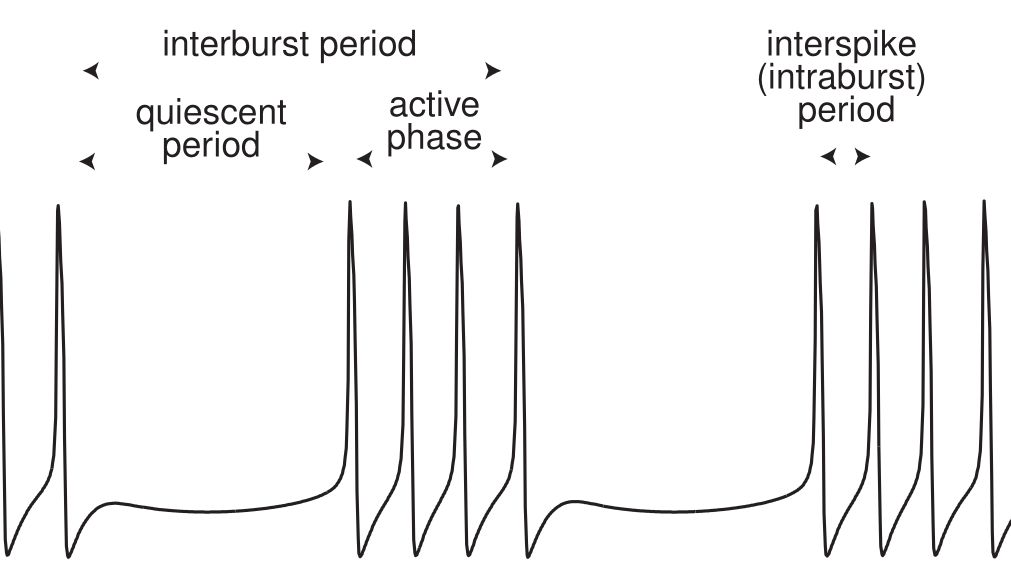
\includegraphics[height=.85\textheight]{./burster.png}
\end{center}
\end{frame}

\begin{frame}[label={sec:org648af70}]{Rinzel's burster analysis}
Consider the system

\[ \dot{x} = f(x,y) ~FAST,\]
\[ \dot{y} = \varepsilon g(x,y)~SLOW,\]

where 

\[ |\varepsilon| \ll 1~,\] and \[f,g \in \mathcal{O}(1)~.\]
\end{frame}

\begin{frame}[label={sec:org1b669e3}]{Rinzel's burster analysis}
\begin{itemize}[<+->]
\item Consider the singular limit \(\varepsilon \to 0\)
\item The change in \(y\) drops to zero, so \(y\) becomes a constant
\item As \(y\) is now a constant vector, it can be considered as a parameter vector to the fast subsystem
\item Rinzel's approach: consider the bifurcations of the fast subsystem at the singular limit; take the slow subsystem state \(y\) to be a bifurcation parameter, and perform a bifurcation analysis of the fast subsystem with respect to \(y\)
\item Bursting dynamics are then obtained when the slow subsystem dynamics drives the fast subsystem back and forth over one or more bifurcations.
\end{itemize}
\end{frame}

\begin{frame}[label={sec:orga777dec}]{Rinzel's burster analysis}
\begin{columns}
\begin{column}{0.5\columnwidth}
\begin{center}
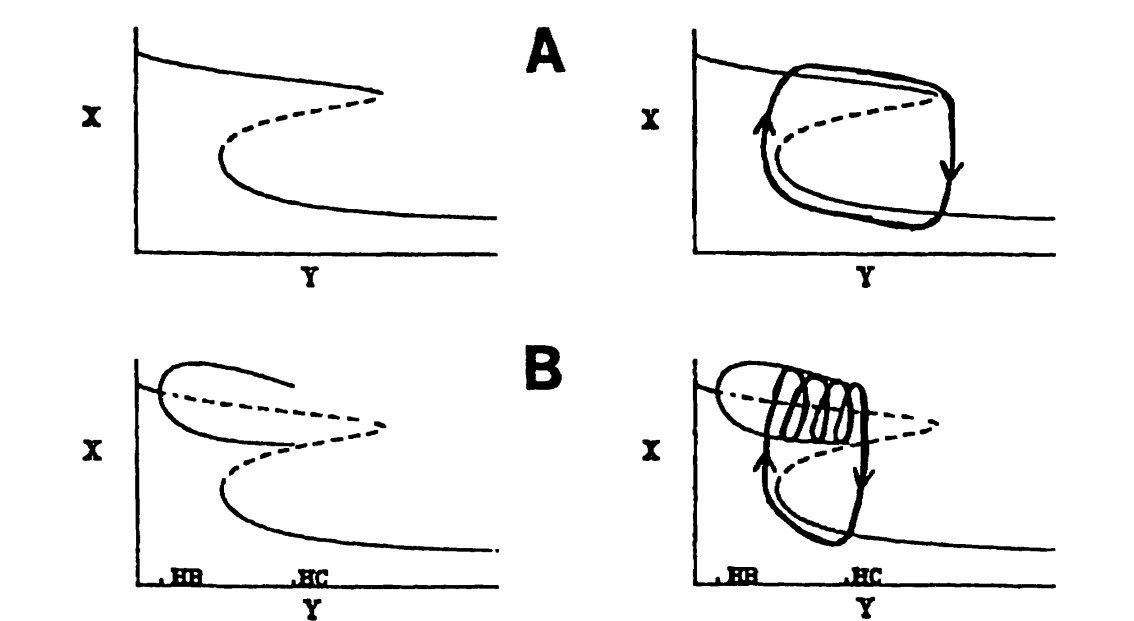
\includegraphics[width=\textwidth]{rinzburst.png}
\end{center}
\end{column}

\begin{column}{0.5\columnwidth}
\begin{center}
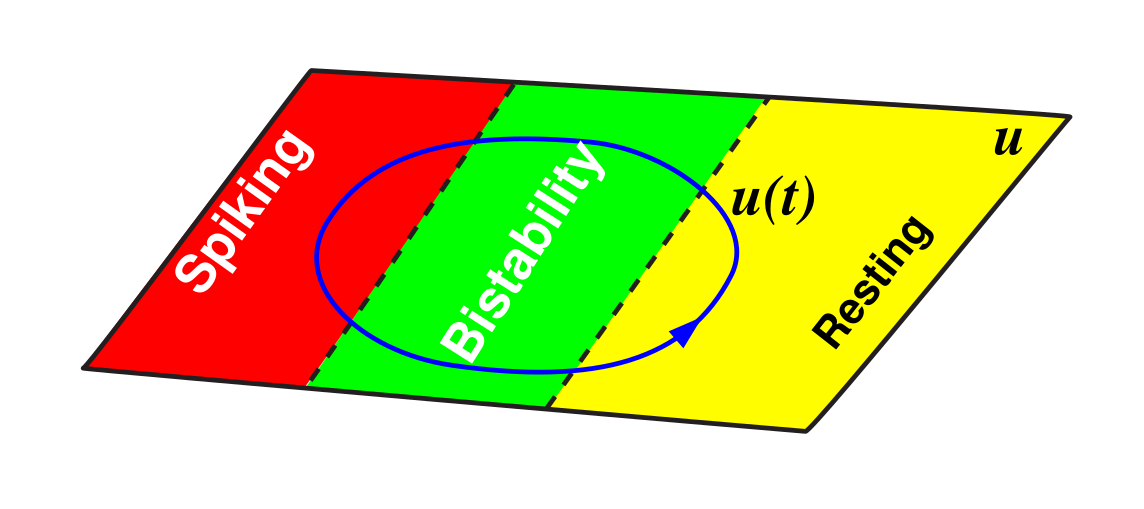
\includegraphics[width=\textwidth]{bursterschematic.png}
\end{center}
\end{column}
\end{columns}
\end{frame}


\section{Burster classification}
\label{sec:org5a7c26c}
\begin{frame}[label={sec:org8688d53}]{Krassy et al.'s paper}
\begin{itemize}
\item Lots of work has been done to classify bursters
\item Krassy's paper seeks to classify the (recently found) psuedo-plateau burster
\item This is achieved by studying the unfolding of a codimension-4 singularity
\item The singularity unfolding could (presumably?) also double up as a generic neuron model
\end{itemize}
\end{frame}

\begin{frame}[label={sec:org3bc2c62}]{Krassy et al.'s paper}
\begin{itemize}
\item Lots of work has been done to classify bursters
\item Krassy's paper seeks to classify the (recently found) psuedo-plateau burster
\item This is achieved by studying the unfolding of a codimension-4 singularity
\item The singularity unfolding could (presumably?) also double up as a generic neuron model
\end{itemize}


The paper builds on the work of Rinzel, Bertram, and Golubitsky (and other less relevant work), briefly recounted as follows.
\end{frame}

\begin{frame}[label={sec:orgbaa2678}]{Classifying bursters - background}
\begin{itemize}
\item Rinzel's work allows for the classification of bursters, according to the bifurcations at either end of the hysteresis loop
\end{itemize}

\begin{columns}
\begin{column}{0.5\columnwidth}
\begin{center}
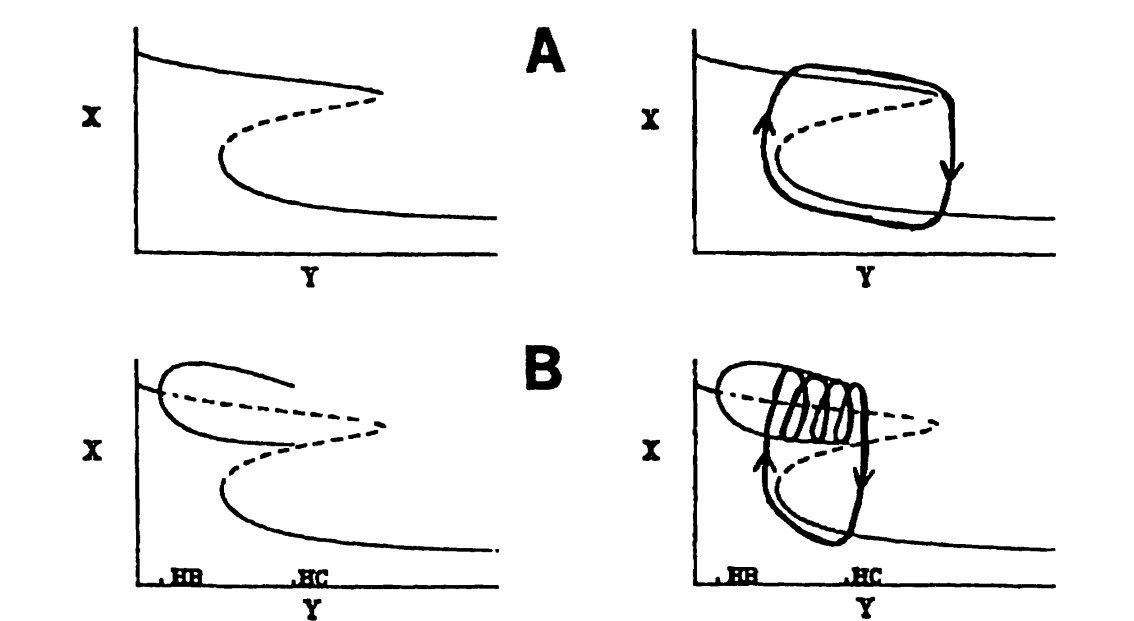
\includegraphics[width=\textwidth]{rinzburst.png}
\end{center}
\end{column}

\begin{column}{0.5\columnwidth}
\begin{center}
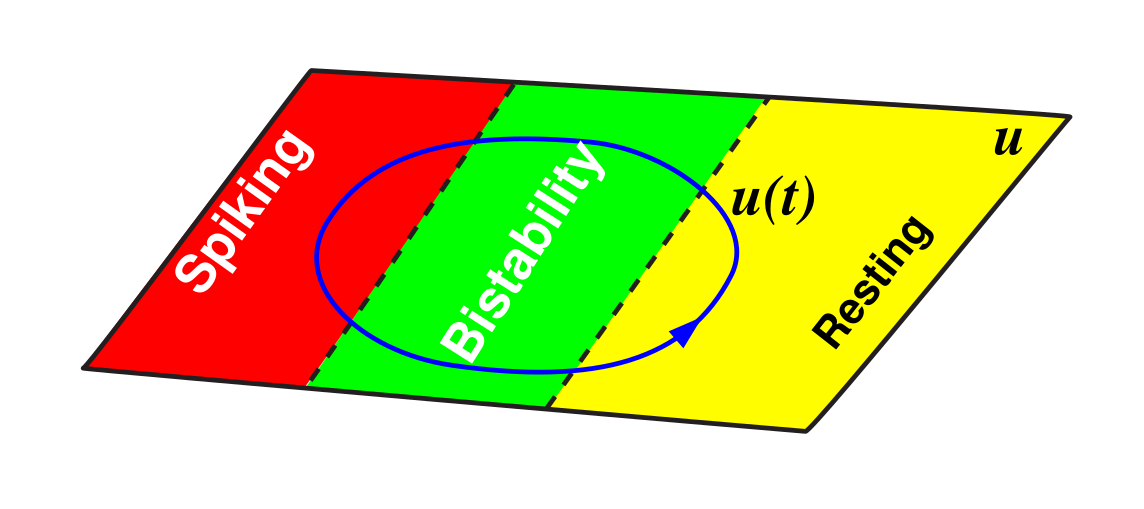
\includegraphics[width=\textwidth]{bursterschematic.png}
\end{center}
\end{column}
\end{columns}
\end{frame}

\begin{frame}[label={sec:org5148b45}]{Classifying bursters - background}
\begin{itemize}[<+->]
\item Rinzel's work allows for the classification of bursters, according to the bifurcations at either end of the hysteresis loop
\item Izhikevich notes that there are four bifurcations that can lead to the onset or termination of bursting, meaning 16 different bursters can exist for a planar fast subsystem
\item Later work decided there's a better way of classifying bursters, in terms of unfoldings of high-codimension singularities
\end{itemize}
\end{frame}

\begin{frame}[label={sec:org4a30350}]{Classifying bursters - Bertram}
\begin{columns}
\begin{column}{0.5\columnwidth}
\begin{itemize}
\item Observation: hysteresis-loop bursters require two bifurcations - one to start spiking, and one to stop it
\item Instead of considering them as isolated bifurcations, consider them as part of the unfolding of a higher-codimension singularity
\end{itemize}
\end{column}

\begin{column}{0.5\columnwidth}
\begin{center}
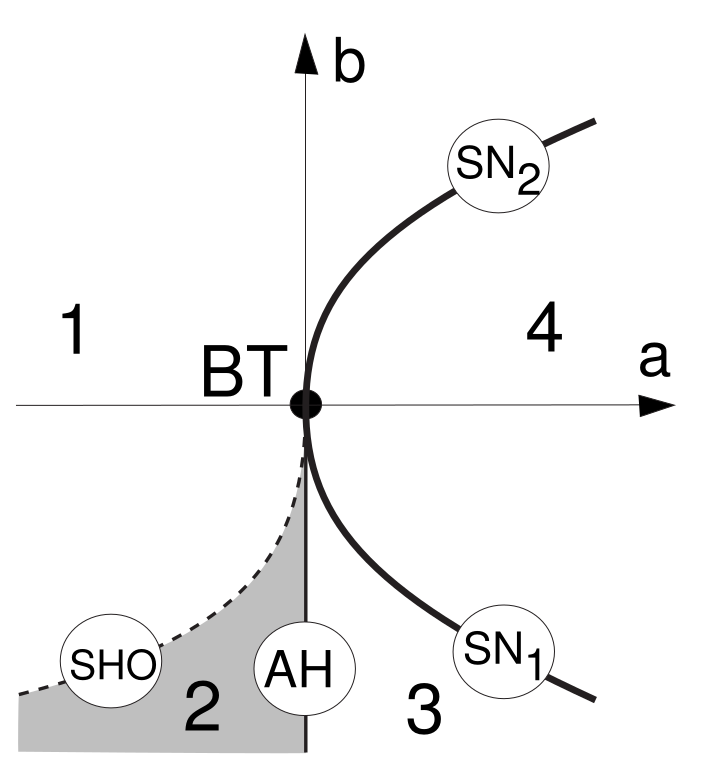
\includegraphics[height=0.8\textheight]{bog.png}
\end{center}
\end{column}
\end{columns}
\end{frame}

\begin{frame}[label={sec:orgf79e540}]{Classifying bursters - Bertram}
\begin{columns}
\begin{column}{0.5\columnwidth}
\begin{itemize}
\item Bursting behaviours are defined by their paths across fast-subsystem bifurcations
\item This is represented as horizontal paths on (here) a two-parameter bifurcation diagram
\item These cuts represent the paths in parameter space that the slow subsystem drives the fast system through
\item Allows for both discovery and classification
\end{itemize}
\end{column}

\begin{column}{0.5\columnwidth}
\begin{center}
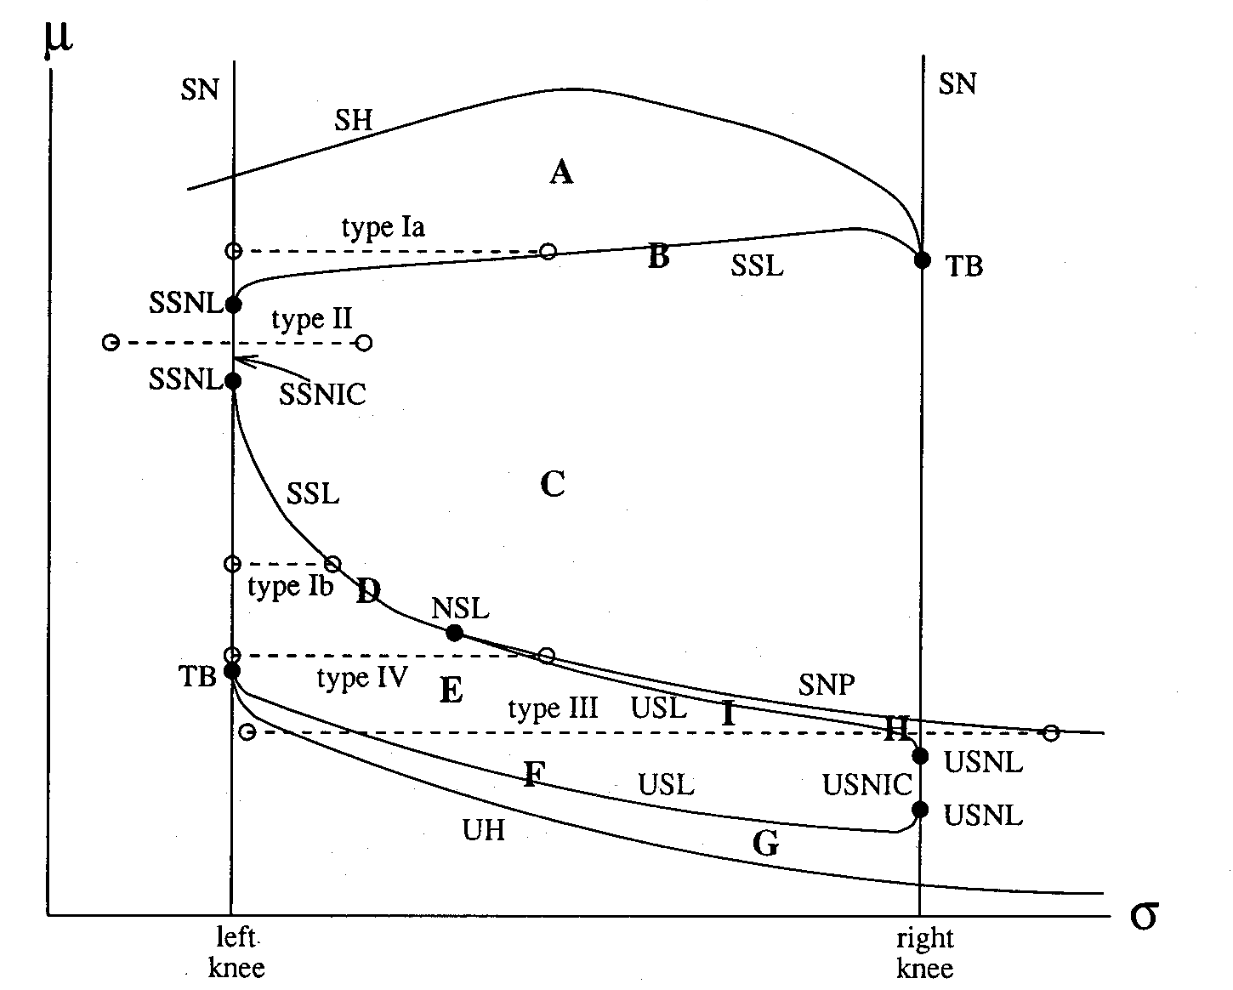
\includegraphics[height=.8\textheight]{bertrambif.png}
\end{center}
\end{column}
\end{columns}
\end{frame}

\begin{frame}[label={sec:orgcf636ee}]{Classifying bursters - Golubitsky}
\begin{itemize}
\item Golubitsky et al. produced a more rigorous version of Bertram's classification
\item The classification is extended to the codimension-3 degenerate Bogdanov-Takens singularity
\item Bursting behaviour later appeared that couldn't be explained as an unfolding of a codim-2 singularity, but could be explained in codim-3
\item The complexity of a burster is defined as the codimension of the singularity in whose unfolding the bursting behaviour first appears; the codim-3 burster would therefore be considered more complex than the codim-2 ones
\end{itemize}
\end{frame}

\begin{frame}[label={sec:org49c7add}]{Classifying bursters - Krassy et al.}
\begin{itemize}
\item Psuedo-plateau bursting is a type of bursting where there's no sustained oscillations in the active phase
\item As far as we know, it can't be explained in terms of codim-3 unfoldings
\item Krassy's paper expands the existing burster classification to include psuedo-plateau bursters
\item A codim-4 doubly-degenerate Bogdanov Takens singularity is shown to include the burster in its unfoldings
\item It is thought to be codim-4, as no codim-3 unfolding is yet known to contain the bursting dynamics
\end{itemize}
\end{frame}


\section{Neuron models}
\label{sec:orge1a1f1c}
\begin{frame}[label={sec:orgdefed81}]{Towards a generic neuron model}
\begin{itemize}
\item The codim-4 unfolding will contain all known bursters (I think?)
\item By ignoring the slow subsystem, we can instead let injected current drive the system across a bifurcation (not necessarily in a biologically plausible way)
\item The model will therefore be able to demonstrate all the bifurcations a non-bursting neuron can undergo
\item This makes it a potential candidate for a generic model
\end{itemize}
\end{frame}

\begin{frame}[label={sec:orgcb6378d}]{Towards a generic neuron model}
\begin{itemize}[<+->]
\item Bursters in Krassy's paper are driven by a sinusoidal forcing term
\item This means the slow subsystem must be self-oscillating (called a slow-wave burster)
\item We can also have resonant slow subsystems, which don't oscillate on their own (hysteresis-loop bursters, acting in similar ways to Fitzhugh-Nagumo)
\item To model all neuron types (inc. hysteresis- and slow-wave bursters), we need a different slow subsystem model
\item I've found a paper (ref below) that builds extensively on Krassy's paper to develop such a model
\item It is designed to model just about every single neuron that's likely to exist, making it another good generic neuron model
\end{itemize}
\end{frame}


\section{Next steps}
\label{sec:org675a7bb}
\begin{frame}[label={sec:orgf2e9416}]{Next steps}
\begin{itemize}
\item I don't really understand the bifurcations of Krassy's neuron model, so work on achieving that
\item Read paper about the generic neuron model, and its bifurcations
\item Decide which bifurcations to test myself
\item Use XPP etc. to do a bifurcation analysis on the model
\item Use those analyses to produce a software comparison paper
\item Also, look at networks of neurons and their models, dynamics, bifurcations, etc.
\item Then, start learning about control strategies
\end{itemize}

\emph{Saggio, Maria Luisa, et al. "Fast–Slow Bursters in the Unfolding of a High Codimension Singularity and the Ultra-slow Transitions of Classes." The Journal of Mathematical Neuroscience 7.1 (2017): 7.}


\end{frame}
\begin{frame}[plain]
\begin{center}
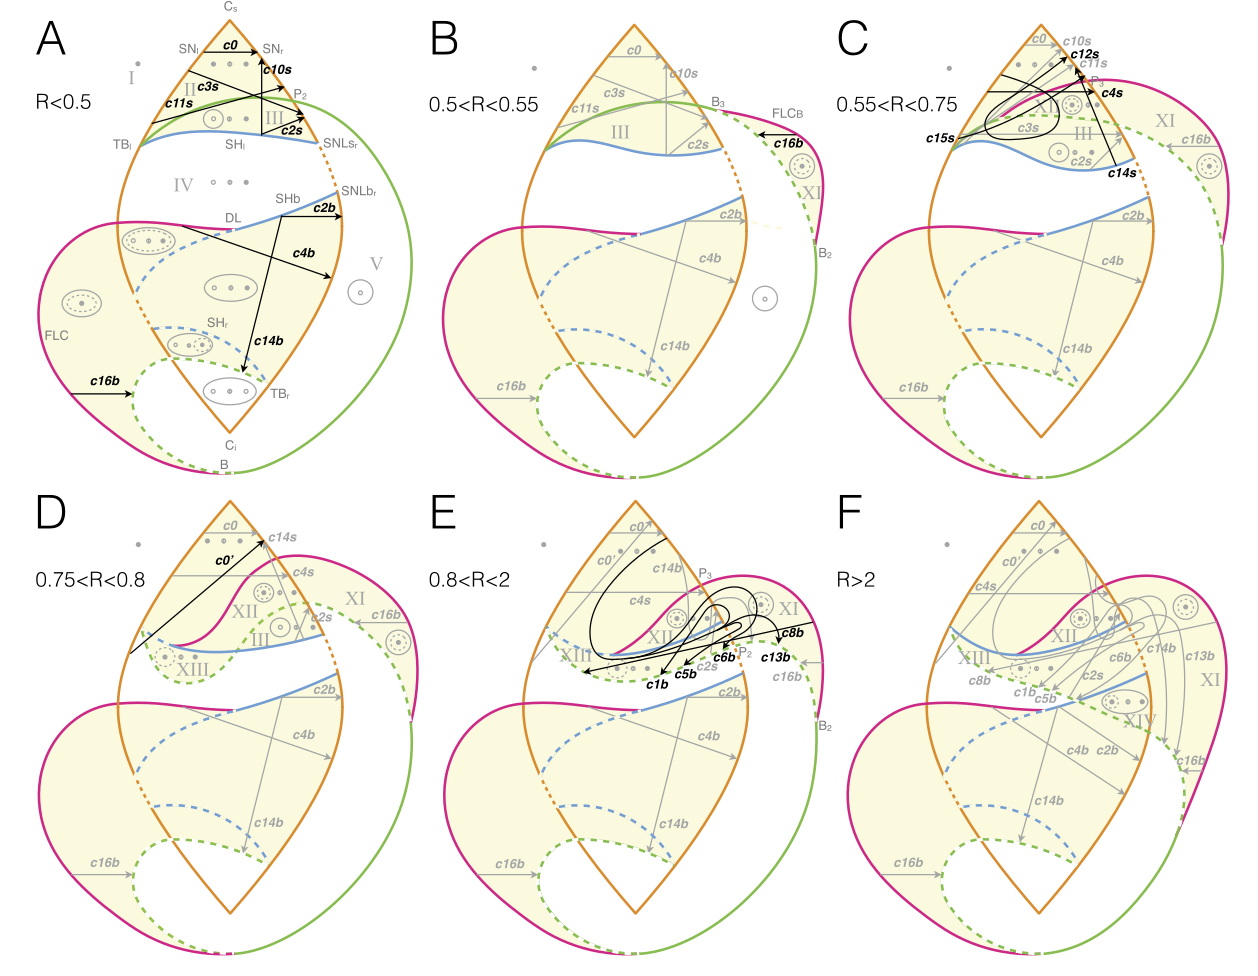
\includegraphics[height=1.3\textheight]{hardbif.png}
\end{center}
\end{frame}
\end{document}
